\documentclass{beamer}

\usepackage[T1]{fontenc}
\usepackage[utf8]{inputenc}
\usepackage[italian, english]{babel}

\usepackage{comment} 		% Use comment env

\usepackage{amsmath}
\usepackage{amssymb}
\usepackage{amsthm}
\usepackage{enumerate} 					% Lists
\usepackage{float}
\usepackage{graphicx}					% Insert figures
\usepackage{subfig}						% More figures together
\usepackage{mathtools}
\usepackage{stmaryrd}
\usepackage{tikz-cd} 					% Diagrams
\usepackage{verbatim}
\usepackage{lipsum} 					% Write garbage

%%% abs and norm %%%
\DeclarePairedDelimiter\abs{\lvert}{\rvert}%
\DeclarePairedDelimiter\norm{\lVert}{\rVert}%

% Swap the definition of \abs* and \norm*, so that \abs
% and \norm resizes the size of the brackets, and the 
% starred version does not.
\makeatletter
\let\oldabs\abs
\def\abs{\@ifstar{\oldabs}{\oldabs*}}

\let\oldnorm\norm
\def\norm{\@ifstar{\oldnorm}{\oldnorm*}}
\makeatother

% New math operators
\DeclareMathOperator{\Ima}{Im}			% Write Im of a function in math mode
\DeclareMathOperator{\dist}{ dist }		% Write dist(A, B) between sets
\DeclareMathOperator{\Log}{Log} 		% Iwasawa continuation of log_p
\DeclareMathOperator{\card}{card}		% Cardinality of a set

% New commands
\newcommand{\N}{ \mathbb{N} }
\newcommand{\Nb}{ \mathbf{N} }
\newcommand{\Z}{ \mathbb{Z} }
\newcommand{\Q}{ \mathbb{Q} }
\newcommand{\R}{ \mathbb{R} } 
\newcommand{\C}{ \mathbb{C} }
\newcommand{\F}{ \mathbb{F} }
\newcommand{\E}{ \mathrm{E} } % Artin-Hasse exponential
\newcommand{\Zp}{ \Z_p }
\newcommand{\Qp}{ \Q_p }
\newcommand{\Fp}{ \F_p }
\newcommand{\Cp}{ \C_p }
\newcommand{\padic}{$p$-adic }
\newcommand{\Qpa}{ \Qp^{\textup{alg cl} } }
\newcommand{\Qpu}{ \Qp^{\textup{unram}  } }
\newcommand{\Zpu}{ \Zp^{\textup{unram}  } }
\newcommand{\ord}{ \textrm{ord}_p\, }  %%% \, is a slight space %%%
\newcommand{\pabs}[1]{ \abs{#1}_p }
\newcommand{\ser}[1]{ \llbracket {#1} \rrbracket } % Write quickly formal power series
\newcommand{\newt}[1]{ \mathfrak{N}(#1) } % Write quickly the Newton polygon of f

% Renewed commands
\renewcommand{\phi}{\varphi}
\renewcommand{\epsilon}{\varepsilon}
\renewcommand{\hat}{\widehat}
\renewcommand{\tilde}{\widetilde}

% Theorem styles
\theoremstyle{plain}
\newtheorem{prop}{Proposition}


\title[\padic analysis]{Analytic functions on \padic fields}
\author[Carlo Buccisano]{Laureando: Carlo Buccisano\\Relatore: Prof. Maurizio Cailotto}
\date[5 luglio 2019]{5 luglio 2019\\Anno Accademico 2018/2019}
\institute[Università di Padova]{Corso di laurea triennale\\Dipartimento di Matematica ``Tullio Levi-Civita''\\Università degli Studi di Padova}
\logo{
\includegraphics[scale=0.1]{/home/carlo/Tesi/images/sigillo_unipd}}

\usetheme{Warsaw}
%\usecolortheme{beaver}
\useoutertheme{infolines}
\setbeamercovered{transparent}

\beamertemplatenavigationsymbolsempty % Remove navigation bar 
\setbeamertemplate{headline}{}


\begin{document}
	% Title
	\begin{frame}
		\maketitle
	\end{frame}
	
	% Remove logo
	\logo{} 
	
	% Planning
	\begin{frame}
		\frametitle{Plan of the presentation}
		\tableofcontents[pausesections]
	\end{frame}
	
	% Introduction
	\section{Basic Concepts}
	\begin{frame}
		\frametitle{Field norms}
		\begin{definition}
			Let $F$ be a field, a function $\norm{\ }\colon F \to \R_{\geq 0}$ is a \alert{field norm} if:
			\begin{enumerate}
				\item $\norm{x} = 0 \iff x = 0$;
				\item $\norm{x \cdot y} = \norm{x} \cdot \norm{y}$;
				\item $\norm{x + y} \leq \norm{x} + \norm{y}$.
			\end{enumerate}
		\end{definition}
		\pause
		\begin{definition}
			Let $F$ be a field and $\norm{\ }_1, \norm{\ }_2$ two field norms. They are said to be equivalent if they have the same Cauchy sequences.
		\end{definition}
		\pause
		\begin{example}
			The classic absolute value $\abs{\ }_{\infty}$ is a field norm on $\Q$.
		\end{example}
	\end{frame}
	\begin{frame}
		\frametitle{Non-Archimedean field norms}
		\begin{definition}
			Let $F$ be a field and $\norm{\ }\colon F \to \R_{\geq 0}$ a field norm. We say that $\norm{\ }$ is a \alert{non-Archimedean} norm if, for every $x, y \in F$, we have
			\[
				\norm{x + y} \leq \max\left\{\norm{x}, \norm{y}\right\}.
			\]
		\end{definition}
		\pause
		An immediate consequence is the following.
		\begin{prop}
			With $(F, \norm{\ })$ as before, we have:
			\[
				\norm{x} \neq \norm{y} \implies \norm{x + y} = \max\left\{\norm{x}, \norm{y}\right\}.
			\]
		\end{prop}
		It can be proved that every triangle in such a space is isosceles.
	\end{frame}

	\section{Construction of $\Qp$: analytic approach}
	\begin{frame}
		\frametitle{\padic order}
		Let $p$ be a fixed prime number.
		\begin{definition}
			Let's define a function $\ord\colon \Z \to \N \cup \{+\infty\}$ as follows:
			\begin{gather*}
				\ord a :=
				\begin{cases}
					+\infty, & \text{if $a = 0$;}\\
					n, & \text{such that $p^n \mid a$ and $p^{n+1} \nmid a$.}
				\end{cases}.
			\end{gather*}
			We can extend it to $\Q$ setting $\ord\left(\tfrac{a}{b}\right) := \ord a - \ord b$.
		\end{definition}
		\pause
		\begin{prop}
			The function $\mathrm{ord}_p\colon \Q \to \Z\cup\{+\infty\}$ is a discrete valuation.
		\end{prop}
	\end{frame}
	\begin{frame}
		\frametitle{\padic absolute value}
		Finally we can define the \padic absolute value.
		\begin{definition}
			The function $\pabs{\ }\colon \Q \to \Q$ defined by
			\begin{gather*}
				\pabs{x} :=
				\begin{cases}
					p^{-\ord x}, & \text{if $x \neq 0$;}\\
					0, & \text{otherwise;}
				\end{cases}
			\end{gather*}
			is the \padic absolute value on $\Q$. 
		\end{definition}
		\pause
		\begin{prop}
			The \padic absolute value is a non-Archimedean field norm on $\Q$.
		\end{prop}
	\end{frame}
	\begin{frame}
		\frametitle{Ostrowski theorem}
		\begin{definition}
			The function $\abs{\ }_0\colon \Q \to \R_{\geq 0}$ defined by 
			\begin{gather*}
				\abs{x}_0 :=
				\begin{cases}
					1, & \text{if $x \neq 0$;}\\
					0, & \text{otherwise.}
				\end{cases}
			\end{gather*}
			is the \alert{trivial norm}.
		\end{definition}
		\pause
		\begin{theorem}[Ostrowski]
			Every non-trivial norm on $\Q$ is equivalent to $\pabs{\ }$ where $p = \infty$ or is some prime number.
		\end{theorem}
	\end{frame}
	\begin{frame}
		\frametitle{Definition of $\Qp$}
		It can be proved (using Hensel's lemma) that:
		\begin{prop}
			The space $(\Q, \pabs{\ })$ is not complete.
		\end{prop}
		\pause
		\begin{definition}
			The completion of $(\Q, \pabs{\ })$ is the space $(\Qp, \pabs{\ })$, obtained considering $\mathcal{S}$, the set of all the Cauchy sequences, and identifying $(a_n)_n$ and $(b_n)_n$ if $\lim_{n \to +\infty }\pabs{a_n - b_n} = 0$. 
		\end{definition}
		It can be proved that, with component-wise sum and product, $\Qp$ is actually a field containing $\Q$. 
	\end{frame}
	\begin{frame}
		\frametitle{Structure of $\Qp$}
		\begin{prop}
			The \padic absolute value can be extended to $\Qp$ setting 
			\[
			\pabs{a} := \lim_{n \to +\infty} \pabs{a_n},
			\]
			where $(a_n)_{n \in \N}$ is any representative of $a$.
		\end{prop}
		\pause
		\begin{theorem}
			For every $a \in \Qp$ there exists a unique representation as 
			\[
				a = \sum_{i=m}^{+\infty} a_ip^i, \qquad m \in \Z, a_i \in \{0, \dots, p-1\}.
			\]
		\end{theorem}
	\end{frame}
	\begin{frame}
		\frametitle{Representation of $\Q$ in $\Qp$}
		Clearly, if $a \in \Qp^{\times}$, we have $\pabs{a} = p^{-\ord a}$, where $\ord a$ is the index of the first non-zero coefficient in $a$.
		\begin{prop}
			Given $a = \sum_{i=m}^{+\infty} a_ip^i \in \Qp$ we have 
			\[
				a \in \Q \iff \exists r, N \in \N : a_i = a_{i+r} \,\forall i > N
			\]
		\end{prop}
		\pause
		It's then easy to note that $\Q$ is dense in $\Qp$.
		\begin{example}
			The \padic number $\alpha := \sum_{i=0}^{+\infty} p^{2^i}$ hasn't a periodic expansion so $\alpha \in \Qp \setminus \Q$. 
		\end{example}
	\end{frame}
	
	\section{Construction of $\Qp$: algebraic approach}
	\begin{frame}
		\frametitle{Definition of $\Zp$}
		We can obtain $\Qp$ using a more algebraic construction, which will highlight some other important properties.
		\begin{definition}
			A \padic integer is a formal series $\sum_{i=0}^{+\infty} a_ip^i$, with integer coefficients $0 \leq a_i \leq p-1$. The set containing all the \padic integers is called $\Zp$.
		\end{definition}
		\pause
		\begin{prop}
			The set $\Zp$ equipped with a component-wise sum and a Cauchy product (both with carry) is a characteristic $0$ integral domain.
		\end{prop}
	\end{frame}
	\begin{frame}
		\frametitle{Properties of $\Zp$}
		It's immediate that the invertible elements of $\Zp$ are exactly the ones with a non-zero constant term. 
		\begin{prop}
			$\Zp$ is a topological ring (sum and multiplication are continuous) and a principal ideal domain, whose ideals are $\{0\}$ and $p^k\Zp$, with $k \in \N$.
		\end{prop}
		\pause
		\begin{prop}
			$\Zp$ is a compact space and is exactly the completion of $(\Z, \pabs{\ })$.
		\end{prop}
	\end{frame}
	\begin{frame}
		\frametitle{Projective limits}
		\begin{definition}
			A sequence $(E_n, \phi_n)_{n \in \N}$ of sets and maps $\phi_n\colon E_{n+1} \to E_n$ is called a projective system.	A set $E$ equipped with maps $\psi_n\colon E \to E_n$ such that $\psi_n = \phi_n \circ \psi_{n+1}$, is called a \alert{projective limit} of the system if every compatible set of maps can be factorized through it. It can be proved that $E$ is unique, up to bijections, and it's often called $\lim\limits_{\longleftarrow} E_n$.
		\end{definition}
		\pause
		\begin{theorem}
			Let's consider the projective system $(\Z/p^n\Z, \pi_n)$ where $\pi_n\colon \Z/p^{n+1}\Z \to \Z/p^n\Z$ is the classical projection and let $\lim\limits_{\longleftarrow}\Z/p^n\Z$ be its projective limit. Then $\Zp$ and $\lim\limits_{\longleftarrow}\Z/p^n\Z$ are two isomorphic topological rings.
		\end{theorem}
	\end{frame}
	\begin{frame}
		\frametitle{Projective limits}
		The universal factorization property is the following: for every compatible sequence of maps $(f_n)_n$, i.e. $f_n\colon X \to E_n$ and $f_n = \phi_n \circ f_{n+1}$, there exists $f\colon X \to \lim\limits_{\longleftarrow}E_n$ such that $f_n = \psi_n \circ f$.
		\begin{equation*}
			\begin{tikzcd}[ampersand replacement=\&, row sep = large, column sep = large]
				\& \& \& \& \lim\limits_{\longleftarrow}E_n  \arrow[dlll, "\psi_n"']  \arrow[dll, "\psi_{n+1}"]	\\
				\dots \& \arrow[l] E_n \& \arrow[l, "\varphi_n"] E_{n+1} \& \arrow[l] \dots \\
				\& \& \&  \& X \arrow[ulll, "f_n"]  \arrow[ull, "f_{n+1}"'] \arrow[uu, dashed, "f"]
			\end{tikzcd}
		\end{equation*}
	\end{frame}
	\begin{frame}
		\frametitle{Another definition of $\Qp$}
		\begin{prop}
			The field $\Qp$ is exactly the field of fractions of $\Zp$.
		\end{prop}
		Let's observe that, with this construction, the structure of $\Qp$ is immediate.
		\pause
		\begin{example}[Geometric series]
			Let's consider $\sum_{i=0}^{+\infty} p^i \in \Zp$. This series doesn't converge in $(\Q, \abs{\ }_{\infty})$ but, in $(\Q, \pabs{\ })$, we have $\lim_{i \to +\infty} p^i = 0$ so it converges and we have
			\[
				\sum_{i=0}^{+\infty} p^i = \frac{1}{1 - p} \implies \left(\sum_{i=0}^{+\infty}p^i\right)^{-1} = 1 - p.
			\]
		\end{example}
	\end{frame}
	\begin{frame}
		\frametitle{Hensel's lemma}
		\begin{theorem}[Hensel's lemma]
			Let $P(X) \in \Zp[X]$ and $x \in \Zp$ such that $P(x) \equiv 0 \mod p^n$. If $k := \mathrm{ord}_p\,(P'(x)) < n/2$ then there exists a unique $\xi \in \Zp$ such that $\xi \equiv x \mod p^{n - k}$ and $P(\xi) = 0$.
		\end{theorem}
		Using this powerful tool we can prove the aforementioned non-completeness of $(\Q, \pabs{\ })$.
		\pause
		\begin{example}
			We just need to find a suitable polynomial with no roots in $\Q$ but a root in $\Z/p\Z$.
			\begin{itemize}
				\item For $p = 2$: $P(X) = X^3 - 7$.
				\item For $p=3$: $P(X) = X^2 - 7$.
				\item For $p \equiv 1 \mod 4$: $P(X) = X^2 - (p+1)$.
				\item For $p \equiv 3 \mod 4$: $P(X) = X^2 - t$, where $4t \equiv 1 \mod p$.
			\end{itemize}
		\end{example}
	\end{frame}
	
	\section{Finite field extensions of $\Qp$}
	\begin{frame}
		\frametitle{Extension of the \padic absolute value}
		\begin{prop}
			Let $V$ be a finite dimensional $\Qp$-vector space. Then all norms on $V$ are equivalent.
		\end{prop}
		It's then easy to prove that if $K/\Qp$ is a finite degree field extension then there can be at most one field norm on $K$ extending the \padic one.
		\pause
		\begin{theorem}
			Let $K/\Qp$ be a field extension of degree $d < +\infty$. Then there is a unique extension of the \padic absolute value to $K$ and is obtained setting
			\[
				\pabs{x} := \pabs{\det \ell_x}^{1/d},
			\]
			where $\ell_x\colon K \to K$ is the linear map $y \to xy$.
		\end{theorem}
	\end{frame}
	\begin{frame} 
		\frametitle{Residue degree and index of ramification}
		\begin{prop}
			Let $K/\Qp$ be a finite field extension and let's define
			\[
				A := \left\{x \in K : \pabs{x} \leq 1 \right\}, \quad M := \left\{x \in K: \pabs{x} < 1\right\}.
			\]
			Then $A$ is the integral closure of $\Zp$ in $K$, $M$ is its maximal ideal and $k := A/M$, the \emph{residue field}, is an extension of $\Fp$ of degree at most $[K : \Qp]$.
		\end{prop}
		\pause
		\begin{definition}
			With the same notations used above, we say that $f := [k : \Fp]$ is the \alert{residue degree} and $e := (\pabs{K^{\times}} : \pabs{\Qp^{\times}})$ is the \alert{ramification index}. It can be proved that $[K : \Qp] = e \cdot f$.
		\end{definition}
	\end{frame}
	\begin{frame}
		\frametitle{Structure of a finite extension}
		\begin{prop}
			Let $K/\Qp$ be a field extension of degree $n = e\cdot f$. Then $K = K_f^{\textup{unram}}(\pi)$, where $K_f^{\textup{unram}}$ is the only totally unramified extension of $\Qp$ of degree $f$ and $	\pi$ is a root of an Eisenstein polynomial in $K_f^{\textup{unram}}[X]$.
		\end{prop}
		\pause
		\begin{theorem}
			Let $K/\Qp$ a finite field extension of degree $n = e\cdot f$ and let $\pi \in K$ such that $\mathrm{ord}_p\,\pi = 1/e$. Then for every $a \in K$ there is a unique representation as
			\[
				a = \sum_{i=m}^{+\infty} a_i\pi^i,
			\]
			where $m = e \cdot \mathrm{ord}_p\,\alpha \in \Z$ and $a_i \in K$ is such that $a_i^{p^f} = a_i$.
		\end{theorem}
	\end{frame}
	
	\section{Construction of $\Cp$}
	\begin{frame}
		\frametitle{Eisenstein's criterion}
		\begin{definition}
			Let $f(X) \in \Zp[X]$ be a monic polynomial of degree $n$ such that
			\[
				f(X) \equiv X^n \mod p, \quad f(0) \not\equiv 0 \mod p^2.
			\]
			Then $f(X)$ is called an \alert{Eisenstein polynomial}.
		\end{definition}
		\begin{theorem}
			If $f(X) \in \Zp[X]$ is an Eisenstein polynomial then it is irreducible in $\Zp[X]$ (and in $\Qp[X]$).
		\end{theorem}
		\pause
		The theorem can be easily generalized: if $K/\Qp$ is a finite extension of degree $n = e\cdot f$ then we can use $\pi$ in place of $p$ (where $\ord \pi = 1/e$), $A$ in place of $\Zp$ and $K$ in place of $\Qp$.
	\end{frame}
	\begin{frame}
		\frametitle{The algebraic closure of $\Qp$}
		\begin{definition}
			The algebraic closure of $\Qp$ is $\Qpa$.
		\end{definition}
		\pause
		\begin{example}
			Let's consider the polynomial $P_n(X) := X^n - p \in \Zp[X]$. It's an Eisenstein's polynomial so it is irreducible in $\Qp[X]$. Then $\Qp$ is not algebraically closed and $[\Qpa : \Qp] = +\infty$.
		\end{example}
		It's clear that there is a (unique) extension of the \padic absolute value to $\Qpa$.
	\end{frame}
	\begin{frame}
		\frametitle{Definition of $\Cp$}
		\begin{theorem}
			$(\Qpa, \pabs{\ })$ is not complete.
		\end{theorem}
		We can then complete it in a standard way (considering all the Cauchy sequences and identifying the ones whose difference tends to zero).
		\begin{definition}
			The completion of $\Qpa$ is called $\Cp$.
		\end{definition}
	\end{frame}
	\begin{frame}
		\frametitle{Properties of $\Cp$}
		\begin{prop}
			$\Cp$ is a field and there is a unique extension of the \padic absolute value, obtained by setting
			\[
				\pabs{x} = \lim_{n \to +\infty} \pabs{x_n},
			\]
			where $(x_n)_n$ is a Cauchy sequence in $\Qpa$ and a representative of $x \in \Cp$.
		\end{prop}
		\pause
		\begin{theorem}
			$\Cp$ is a complete and algebraically closed field.
		\end{theorem}
	\end{frame}
	\begin{frame}
		\frametitle{Structure of $\Cp$}
		\begin{definition}
			Let $r = a/b \in \Q$ with $a \in \Z, b \in \N^{\times}$ and $P(X) = X^b - p^a \in \Qp[X]$. Any root of $P(X)$ in $\Qpa$ is called a \alert{fractional power} and is denoted by $p^r$.
		\end{definition}
		\pause
		\begin{theorem}
			Any non-zero element of $\Cp$ can be written (although not in a unique way) as a product of a fractional power, a root of $1$ and an element in $D_1(1) = \left\{x \in \Cp: \pabs{x - 1} < 1\right\}$.
		\end{theorem}
	\end{frame}
	\begin{frame}
		\frametitle{Other properties of $\Cp$}
		\begin{prop}
			We have the following properties:
			\begin{itemize}[<+->]
				\item $\pabs{\Cp} = \pabs{\Qpa} = p^{\Q} \cup \{0\}$;
				\item $\card(\Cp) = \card(\R)$;
				\item there exists a (non-canonical) field isomorphism between $\C$ and $\Cp$.
			\end{itemize}
		\end{prop}
	\end{frame}
	\begin{frame}
		\frametitle{A comparison with the classical case}
		The following diagram shows the differences between the construction of $\C$ and $\Cp$ (in-fact they are simply the smallest complete and algebraically closed fields containing $\Q$ with respect to $\abs{\ }_{\infty}$ and $\pabs{\ }$, respectively).
		\begin{equation*}
			\begin{tikzcd}[ampersand replacement=\&]
			\& \R \arrow[r, "\text{alg cl}"] \& \C \\
			\Q \arrow[ur, "\abs{\ }_{\infty}"] \arrow[dr, "\pabs{\ }"'] \\
			\& \Qp \arrow[r, "\text{alg cl}"] \& \Qpa \arrow[r, "\pabs{\ }"] \& \Cp
			\end{tikzcd}
		\end{equation*}
	\end{frame}
	\begin{frame}
		\frametitle{A comparison with the classical case}
		From the previous diagram, it seems that the \padic case is much more complicated than the classic one. Actually, we could have gotten to $\C$ (and $\Cp$) with the same number of steps:
		\begin{equation*}
			\begin{tikzcd}[ampersand replacement=\&]
			\& \&  \C \\
			\Q \arrow[r, "\textup{alg cl}"] \& \Q^{\textup{alg cl}} \arrow[ur, "\abs{\ }_{\infty}"] \arrow[dr, "\pabs{\ }"'] \\
			\& \& \Cp
			\end{tikzcd}
		\end{equation*}
		but the problem is that $\Q^{\textup{alg cl}}$ is a very difficult field to study.
	\end{frame}

	\section{\padic power series}
	\begin{frame}
		\frametitle{Basic properties}
		Let's recall some basic properties of ultrametric complete spaces (we state them for $\Cp$ but they can be generalized).
		\begin{prop}
			\begin{itemize}[<+->]
				\item A sequence $(x_n)_{n \in \N} \subset \Cp$ is Cauchy if and only if $\lim_{n \to +\infty} \pabs{x_{n+1} - x_n} = 0$.
				\item A series $\sum_{i=0}^{+\infty} c_i$ converges in $\Cp$ if and only if $\lim_{i \to +\infty} c_i = 0$.
				\item If $\sum_{n=0}^{+\infty} a_n$ converges then its terms can be re-arranged in any way.
				\item If $a_1 + a_2 + \dots + a_n = 0$ then there exists $i \neq j$ such that $\pabs{a_i} = \pabs{a_j} = \max_{1 \leq h \leq n} \pabs{a_h}$.
			\end{itemize}
		\end{prop}
	\end{frame}
	\begin{frame}
		\frametitle{The main idea}
		The main idea used to prove the next propositions on analytic function is this:
		\begin{theorem}
			Let $f(X_1, \dots, X_n) \in \C\ser{X_1, \dots, X_n}$ be a power series, absolutely convergent on $[-\epsilon, \epsilon]^n \subset \R^n$ for some $\epsilon > 0$. If for every $x_1, \dots, x_n \in [-\epsilon, \epsilon]$ we have $f(x_1, \dots, x_n) = 0$ then $f$ is identically zero.
		\end{theorem} 
	\end{frame}
	\begin{frame}
		\frametitle{Analytic functions}
		\begin{definition}
			A (partial) function $f\colon \Cp \to \Cp$ is an \alert{analytic function} if 
			\[
				f(X) := \sum_{n=0}^{+\infty} a_nX^n, \quad a_i \in \Cp.
			\]
		\end{definition}
		\pause
		\begin{prop}
			Using the same notations, the radius of convergence of $f$ is given by:
			\[
				r = \frac{1}{\limsup \pabs{a_n}^{1/n}}.
			\]
		\end{prop}
	\end{frame}
	\begin{frame}
		\frametitle{Analytic functions}
		Clearly if $\pabs{x} < r$ then $f$ converges, if $\pabs{x} > r$ then $f$ diverges. The behaviour when $\pabs{x} = r$ depends on $f$: $f$ can either converge or diverge on the whole border.
		\begin{prop}
			If $f(X) = \sum_{n=0}^{+\infty} a_nX^n$ converges on some disc $D$, then $f$ is continuous on $D$.
		\end{prop}
		\pause
		\begin{prop}
			Every $f(X) \in \Zp\ser{X}$ converges on $D(1^-) := \left\{x \in \Cp : \pabs{x} < 1 \right\}$.
		\end{prop}
	\end{frame}
	\begin{frame}
		\frametitle{\padic logarithm}
		\begin{definition}
			The function defined by
			\[
				\log_p(X) := \sum_{n=1}^{+\infty} (-1)^{n+1}\frac{(X - 1)^n}{n}
			\]
			is called the \alert{\padic logarithm}. It can be proved that it converges on $D_1(1^-)$ and diverges elsewhere.
		\end{definition}
		\pause
		\begin{prop}
			We have
			\[
				\log_p(x\cdot y) = \log_p(x) + \log_p(y), \quad \forall x, y \in D_1(1^-).
			\]
		\end{prop}
	\end{frame}
	\begin{frame}
		\frametitle{\padic exponential}
		\begin{definition}
			The function defined by
			\[
			\exp_p(X) := \sum_{n=0}^{+\infty} \frac{X^n}{n!}
			\]
			is called the \alert{\padic exponential}. It can be proved that it converges on $D(r_p^-)$ and diverges elsewhere, where $r_p := p^{-1/(p-1)} < 1$.
		\end{definition}
		\pause
		\begin{prop}
			We have
			\[
				\exp_p(x + y) = \exp_p(x) \cdot \exp_p(y), \quad \forall x, y \in D(r_p^-).
			\]
		\end{prop}
	\end{frame}
	\begin{frame}
		\frametitle{\padic exponential and logarithm}
		\begin{theorem}
			The restrictions $\log_p\colon D_1(r_p^-) \to D(r_p^-)$ and $\exp_p\colon D(r_p^-) \to D_1(r_p^-)$ are two mutually inverse isomorphisms between the multiplicative group $(D_1(r_p^-), \cdot)$ and the additive group $(D(r_p^-), +)$.
		\end{theorem}
	\end{frame}
	\begin{frame}
		\frametitle{\padic binomial expansion}
		\begin{definition}
			Fixed $a \in \Cp$, the function defined by
			\[
				B_{a,\,p}(X) := \sum_{n=0}^{+\infty} \binom{a}{n}X^n = 1 + \sum_{n=1}^{+\infty} \frac{a(a-1)\cdots(a-n+1)}{n!}X^n
			\]
			is called the \alert{\padic binomial expansion}.
		\end{definition}
		\pause
		\begin{prop}
			If $\pabs{a} > 1$ then the region of convergence of $B_{a,\,p}(X)$ is $D((r_p/\pabs{a})^-)$. If $\pabs{a} \leq 1$ then $B_{a,\,p}(X)$ converges on $D(r_p^-)$. Finally, if $a \in \Zp$ then $B_{a,\,p}(X) \in \Zp\ser{X}$.
		\end{prop}
	\end{frame}
	\begin{frame}
		\frametitle{\padic binomial expansion}
		In the classic case, if $\abs{x} < 1$ then $B_a(x)$ is the MacLaurin series of $(1 + x)^a$. There is an analogue in \padic environment.
		\begin{theorem}
			If $a \in \Q^{\times}$ and $x \in \Cp$ is in the region of convergence of $B_{a,\,p}(X)$, then 
			\[
				\left(B_{a,\,p}(x)\right)^{1/a} = 1 + x.
			\]
		\end{theorem}
		In this case we'll sometimes use the shorthand $B_{a,\,p}(X) = (1 + X)^a$.
	\end{frame}
	\begin{frame}
		\frametitle{Achtung!}
		\begin{alertblock}{Remark}
			The same series in $\Q\ser{X}$ can converge to different numbers in $\C$ and in $\Cp$.
		\end{alertblock}
		\pause
		 Let's consider the following example.
		 \begin{example}
		 	\begin{gather*}
		 		B_{1/2}\left(\frac{7}{9}\right) = \frac{4}{3}, \quad 
		 		B_{1/2,\,7}\left(\frac{7}{9}\right) =-\frac{4}{3}
		 	\end{gather*}
		 	In-fact the only square root of $16/9$ which is congruent to $1 \mod 7$ is $-4/3$.
		 \end{example}
	\end{frame}
	\begin{frame}
		\frametitle{Differentiation}
		\begin{definition}
			Let $X \subseteq \Cp$ be a set with no isolated points. A function $f\colon X \to \Cp$ is \alert{differentiable} at $a \in \Cp$ is
			\[
				\exists \lim_{X \ni x \to a} \frac{f(x) - f(a)}{x - a} := f'(a) \in \Cp.
			\]
		\end{definition}
		\pause
		\begin{definition}
			With the same notations used above, let's define this function:
			\[
				\Phi f(x, y) := \frac{f(x) - f(y)}{x - y}.
			\]
			We say that $f$ is \alert{strictly differentiable} at $a \in X$ (and we write $f \in S^1(a)$) if 
			\[
				\Phi f(x, y) \to f'(a)
			\]
			as $(x, y) \to (a, a)$ and $(x, y) \notin \Delta_{X \times X}$.
		\end{definition}
	\end{frame}
	\begin{frame}
		\frametitle{Example of differentiation}
		\begin{theorem}
			Let $f(X) = \sum_{n=0}^{+\infty} a_nX^n$ be an analytic function convergent on some open disc $D$. Then $f$ is strictly differentiable on $D$ and
			\[
				f'(X) = \sum_{n=1}^{+\infty} na_nX^{n-1}.
			\]
		\end{theorem}
		\pause
		\begin{example}
			\[
				\frac{\mathrm{d}}{\mathrm{d}x}\exp_p(x) = \frac{\mathrm{d}}{\mathrm{d}x}\left( \sum_{n=0}^{+\infty} \frac{x^n}{n!} \right) = \sum_{n=1}^{+\infty} \frac{x^{n-1}}{(n-1)!} = \exp_p(x).
			\]
		\end{example}
	\end{frame}
	\begin{frame}
		\frametitle{The Iwasawa logarithm}
		\begin{prop}
			There exists a unique function $\Log_p\colon \Cp^{\times} \to \Cp$ such that:
			\begin{itemize}
				\item $\Log_p(x) = \log_p(x)$ if $x \in D_1(1^-)$;
				\item $\Log_p(x\cdot y) = \Log_p(x) + \Log_p(y)$ for any $x, y \in \Cp^{\times}$;
				\item $\Log_p(p) = 0$.
			\end{itemize}
		\end{prop}
		This is called the \alert{Iwasawa logarithm}.
		\pause
		\begin{prop}
			$\Log_p(X)$ is a locally analytic function with derivative $x \mapsto 1/x$.
		\end{prop}
	\end{frame}
	\begin{frame}
		\frametitle{\padic exponential}
		\begin{definition}
			The function $\mu\colon \N^{\times} \to \N$ defined by
			\begin{gather*}
				\mu(n) :=
				\begin{cases}
					0, & \text{if $n$ is not square-free;} \\
					(-1)^k, & \text{if $n$ is a product of $k$ distinct primes;}
				\end{cases}
			\end{gather*}
			is the \alert{M{\"o}bius function}.
		\end{definition}
		\pause
		\begin{prop}
			We have the following identity in $\Q\ser{X}$:
			\[
				\exp(X) = \prod_{n=1}^{+\infty} B_{-\mu(n)/n}(-X^n) = \prod_{n=1}^{+\infty} (1 - X^n)^{-\frac{\mu(n)}{n}}.
			\]
		\end{prop}
	\end{frame}
	\begin{frame}
		\frametitle{The Artin-Hasse exponential}
		\begin{definition}
			The function defined by
			\[
				\E_p(X) := \prod_{\substack{n = 1 \\ p\, \nmid n}}^{+\infty} B_{-\mu(n)/n,\,p}(-X^n) =  \prod_{\substack{n = 1 \\ p\, \nmid n}}^{+\infty} (1 - X^n)^{-\frac{\mu(n)}{n}}
			\]
			is called the \alert{Artin-Hasse exponential}.
		\end{definition}
		Let's note that we simply removed some terms from the product expression of $\exp_p(X)$. This operation will make $\E_p(X)$ converge on a much bigger disc than $D(r_p^-)$.
	\end{frame}
	\begin{frame}
		\frametitle{The Artin-Hasse exponential}
		\begin{prop}
			We have the following identity in $\Q\ser{X}$:
			\[
				\E_p(X) = \exp_p\left(\sum_{i=0}^{+\infty} \frac{X^{p^i}}{p^i}\right).
			\]
		\end{prop}
		\pause
		\begin{theorem}
			$\E_p(X) \in \Zp\ser{X}$ so it converges on $D(1^-)$.
		\end{theorem}
	\end{frame}
	
	\section{Newton polygon}
	\begin{frame}
		\frametitle{Newton polygon for polynomials}
		\begin{definition}
			Let $f(X) = 1 + \sum_{i=1}^n a_iX^i \in 1 + X\Cp[X]$ be a polynomial of degree $n$. Let's define the set
			\[
				\Gamma := \{(0, 0)\} \cup \left\{(i, \ord a_i) : a_i \neq 0, i \in \{1, \dots, n\} \right\} \subset \R^2.
			\]
			The inferior convex hull of $\Gamma$ in $\R^2$ is the \alert{Newton polygon} of $f(X)$.
		\end{definition}
		\pause
		\begin{columns}
			\begin{column}{0.5\textwidth}
				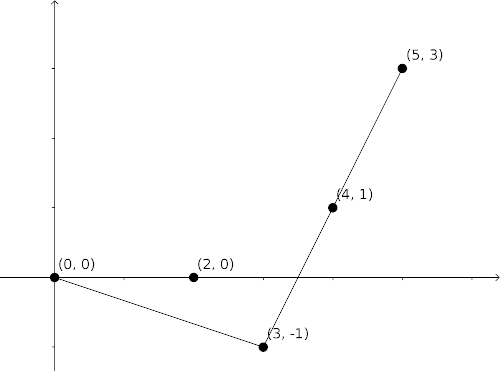
\includegraphics[width=\columnwidth]{/home/carlo/Tesi/images/figure_4_1}
			\end{column}
			\begin{column}{0.5\textwidth}
				The Newton polygon of 
				\[
					f(X) = 1 + X^2 + \tfrac{1}{3}X^3 + 3X^4 + 54X^5
				\]
				in $\Q_3[X]$.
			\end{column}
		\end{columns}
	\end{frame}
	\begin{frame}
		\frametitle{Zeroes of polynomials}
		\begin{definition}
			The \alert{vertices} of the Newton polygon are the points $(j, \ord a_j)$ where the slope changes, while the \alert{segments} are the traits joining every vertex to the next one. The length of a segment is the length of its horizontal projection.
		\end{definition}
		\pause
		\begin{theorem}
			Let $f(X) \in 1 + X\Cp[X]$ be a polynomial of degree $n$ and let $\alpha_1, \dots, \alpha_n$ be all of its roots and $\lambda_i := \mathrm{ord}_p\,(1/\alpha_i)$. If $\lambda$ is a slope of the Newton polygon of length $l$ then precisely $l$ of the $\lambda_i$ are equal to $\lambda$.
		\end{theorem}
		In other words, this theorem says that the slopes of the Newton polygon of $f(X)$ are counting, with multiplicity, the \padic order of the reciprocal roots of $f(X)$.
	\end{frame}
	\begin{frame}
		\frametitle{Newton polygon for power series}
		We can use the same definition of the Newton polygon when $f(X) \in 1 + X\Cp\ser{X}$, which we'll sometimes call $\mathfrak{N}(f)$. We can have three different types of polygons.
		\begin{enumerate}[<+->]
			\item We get infinitely many segments of finite length.
			\item At some point the line we're rotating hits simultaneously infinite points. In this case the Newton polygon has only a finite number of segments, the last one being infinitely long.
			\item At some point the line we're rotating has not hit any point yet but it cannot rotate any farther without passing above some points. In this case the last segment has slope equal to the least upper bound of all possible slopes for which the line passes on or bellow all the points.
		\end{enumerate}
	\end{frame}
	\begin{frame}
		\frametitle{Examples}
		\begin{columns}
			\begin{column}{0.5\textwidth}
				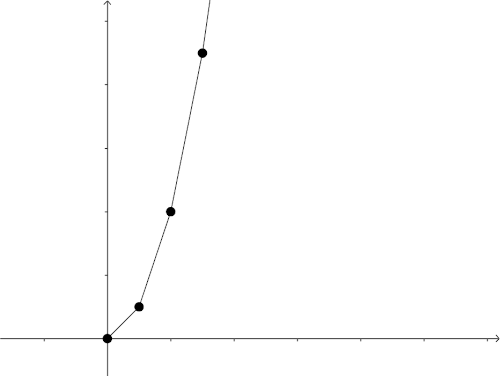
\includegraphics[width=\columnwidth]{/home/carlo/Tesi/images/figure_4_2} \newline
				A type $(1)$ Newton polygon, of
				\[
				f(X) = 1 + \sum_{i=1}^{+\infty} p^{i^2}X^i.
				\] 
			\end{column}
			\begin{column}{0.5\textwidth}
				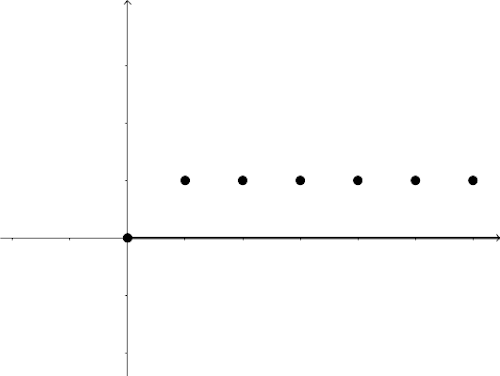
\includegraphics[width=\columnwidth]{/home/carlo/Tesi/images/figure_4_3}
				A type $(3)$ Newton polygon, of
				\[	
				f(X) = 1 + \sum_{i=1}^{+\infty} pX^i.
				\]
			\end{column}
		\end{columns}
	\end{frame}
	\begin{frame}
		\frametitle{A degenerate case}
		There is a degenerate case of type $(3)$: when the line cannot rotate from the beginning. In this case it can be proved that the radius of convergence is always $0$. For example, here's the Newton polygon of $f(X) = \sum_{i=0}^{+\infty} \tfrac{X^i}{p^{i^2}}$.
		\begin{figure}[H]
			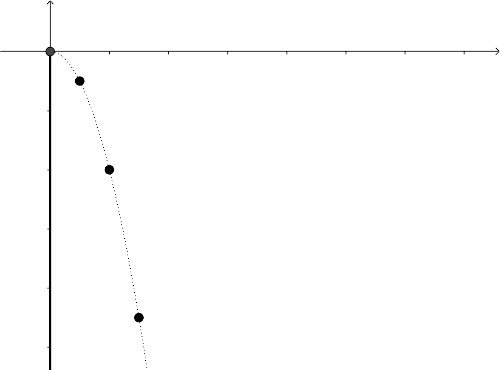
\includegraphics[scale = 1]{/home/carlo/Tesi/images/figure_4_3_1}
		\end{figure}
	\end{frame}
	\begin{frame}
		\frametitle{Radius of convergence}
		\begin{theorem}
			Let $f(X) = 1 + \sum_{i=1}^{+\infty}a_iX^i \in 1 + X\Cp\ser{X}$ be a power series and let $b$ be the least upper bound of all slopes of $\newt{f}$. Then the radius of convergence of $f(X)$ is $r = p^b$ (if $b = +\infty$ then $f(X)$ converges everywhere).
		\end{theorem}
		\pause
		\begin{prop}
			With the same notations used above, $f(X)$ converges on the whole disc $D(p^b)$ if and only if $\newt{f}$ is of type $(3)$ and $\lim_{i \to +\infty}d_i = +\infty$, where $d_i$ is the distance between $(i, \mathrm{ord}_p\, a_i)$ and the last line of $\newt{f}$.
		\end{prop}
	\end{frame}
	\begin{frame}
		\frametitle{Other examples}
		\begin{columns}
			\begin{column}{0.5\textwidth}
				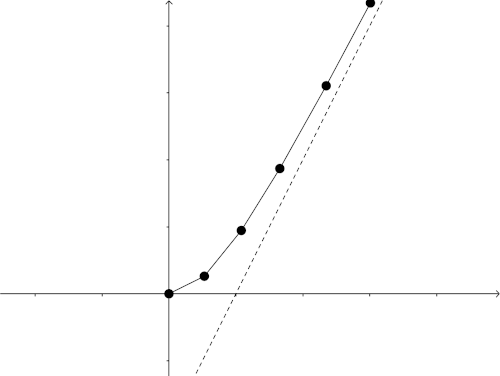
\includegraphics[width=\columnwidth]{/home/carlo/Tesi/images/figure_extra_1} \newline
				There is no convergence at the border.
			\end{column}
			\begin{column}{0.5\textwidth}
				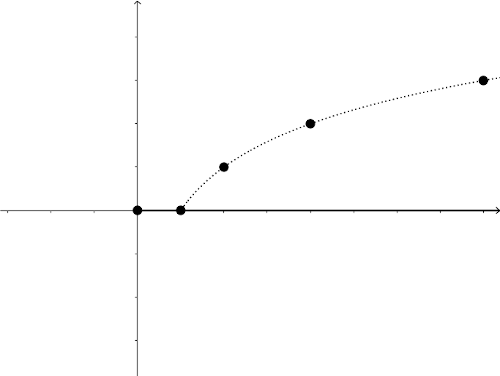
\includegraphics[width=\columnwidth]{/home/carlo/Tesi/images/figure_4_5_1} \newline
				There is convergence at the border.
			\end{column}
		\end{columns}
	\end{frame}
	\begin{frame}
		\frametitle{Weierstrass preparation theorem}
		\begin{theorem}[\padic Weierstrass preparation theorem]
			Let $f(X) = 1 + \sum_{i=1}^{+\infty}a_iX^i$ converge on $D(p^{\lambda})$. Let $N$ be the total horizontal length of all segments in $\newt{f}$ with slope less or equal to $\lambda$, if such number is finite, otherwise let $N$ be the greatest index $i$ such that $(i, \mathrm{ord}_p\,a_i)$ lies on the final segment. Then there exists a polynomial $h(X) \in 1 + X\Cp[X]$ of degree $N$ and a power series $g(X) \in 1 + X\Cp\ser{X}$, which converges and is non-zero on $D(p^{\lambda})$, such that
			\[
				h(X) = f(X) \cdot g(X).
			\]
			The polynomial $h(X)$ is uniquely determined by these properties and $\newt{h}$ coincides with $\newt{f}$ up to $x = N$.
		\end{theorem}
	\end{frame}
	\begin{frame}
		\frametitle{Zeroes of power series}
		From the previous theorem the following proposition is immediate.
		\begin{prop}
			If a segment of $\newt{f}$ has finite length $N$ and slope $\lambda$, then there are exactly $N$ values of $x$ (counting multiplicity) for which $f(x) = 0$ and $\mathrm{ord}_p\,x = -\lambda$.
		\end{prop}
		Clearly every zero of $f(X)$ is obtained in this way. This is the exact power series analogue of the theorem about the zeroes of a polynomial and its Newton polygon.
	\end{frame}
	\begin{frame}
		\frametitle{Applications}
		We can use the Newton polygon to show that the exact region of convergence of $\E_p(X)$ is $D(1^-)$.  We know that
		\[
			\E_p(X) = \exp_p\left(X \cdot f(X)\right),
		\]
		where $f(X) = \sum_{i=0}^{+\infty} \tfrac{X^{p^i - 1}}{p^i}$. The Newton polygon of $f(X)$, using $p=2$, is
		\begin{figure}[H]
			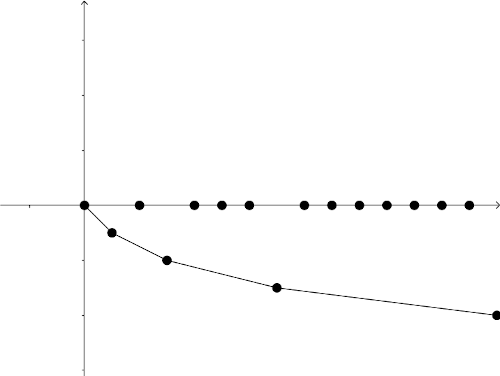
\includegraphics[scale = 1]{/home/carlo/Tesi/images/figure_extra_2}
		\end{figure}
		and it's evident that $r = 1$ and we can't have convergence at border, since $\newt{f}$ is of type $(1)$.
	\end{frame}
	\begin{frame}
		\frametitle{Weierstrass product}
		\begin{theorem}
			Let $f(X) = 1 + \sum_{i=1}^{+\infty} a_iX^i$ be a proper power series (i.e. not a polynomial) everywhere convergent. Then, the set of its zeroes is countable infinite, let it be $(r_n)_{n\geq 1}$, and we have
			\[
				f(X) = \prod_{i=1}^{+\infty} \left(1 - \frac{X}{r_i}\right).
			\]
		\end{theorem}
		\pause
		This theorem implies, in particular, that every non-zero everywhere convergent power series must be a constant. Thus, an exponential like the classic one cannot exist in a \padic environment.
	\end{frame}
\end{document}